\section{Turtlebot Setup for the Project}

The following chapter provides technical details about the hard- and software used to run the robot and control its motion.

\subsection{Turtlebot Configuration}

The Raspberry Pi requires relatively little setup. The official documentation provides a link to the Raspberry Pi \ac{OS} (Raspbian OS). The image includes \ac{ROS} Neotic and can be burned to the SD card via the Raspberry Pi Imager. After a successful boot, the network settings need to be configured to connect to a nearest WiFi. The exact network setup is described in the Network Setup chapter below. After that, it is possible to connect to the Raspberry Pi via \ac{SSH}, which makes further changes to the configuration easier.
The only configuration ROS needs is the IP addresses for both the ROS master and Raspberry Pi itself as well as the Turtlebot model name.

{\scriptsize
\begin{lstlisting}[language=sh,frame=single,caption=Environment Variables,label=code:env]
export ROS_MASTER_URI=http://{IP_ADDRESS_OF_REMOTE_PC}:11311
export ROS_HOSTNAME={IP_ADDRESS_OF_RASPBERRY_PI_3}
export TURTLEBOT3_MODEL=${TB3_MODEL}
\end{lstlisting}}

After that, \lstinline|roslaunch turtlebot3\_bringup turtlebot3\_robot.launch| starts \ac{ROS}, which tries to establish a connection to the remote PC (ROS master). Basic moving operations can be tested with \lstinline|turtlebot3\_teleop\_key| which might run into an error as the default user \enqoute{\textit{ubuntu}} on the Turtlebot image does not have the proper \ac{tty} permissions. The problem can be solved by adding \enqoute{\textit{ubuntu}} to the \enqoute{\textit{root}} user group. This can be done by executing the following command: \lstinline|sudo usermod -aG root ubuntu|. The normal group used for this is called \enqoute{\textit{dialout}} and is not set for \ac{tty}.

The robot is equipped with a Raspberry Pi Cam mounted to the front of the vehicle with a slider to adjust the position of the camera up and down. The slider is necessary to find the optimal position for object detection. A fork with masking tape is mounted to the front of the robot to pick up and hold a tennis ball. The below picture shows the additional modifications to the robot.

\begin{figure}[!ht]
\centering
\includegraphics[width=\linewidth]{images/turtlebot-setup/ball-schubser_front_side_new_desc.jpg}
\caption{Turtlebot Additional Components}
\label{fig:turtlebot-add-components}
\end{figure}

\subsection{Network Setup}

The Raspberry Pi has WiFi capability and is connected to a small home router or alternatively to a mobile phone hotspot. The Docker containers running on the remote PC rely on its host network and thus operate in the same subnet.

\begin{figure}[!htb]
\centering
\includegraphics[width=\linewidth]{images/turtlebot-setup/network_setup.png}
\caption{Network Map used for the Robot Setup}
\label{fig:network-setup}
\end{figure}

\subsection{Containerized Application Setup with Docker}
\label{sec:container-setup}
Docker allows for a simplified setup and development of the robot. Therefore docker runs on the development computer, and the turtlebot connects to the created ROS Nodes.

\begin{figure}[!ht]
\centering
\includegraphics[width=\linewidth]{images/turtlebot-setup/docker-setup.png}
\caption{Development Computer and Turtlebot Setup}
\label{fig:dev-pc-turtlebot}
\end{figure}
%link: https://1drv.ms/u/s!Ar0XPmCdJWduifRsBllZFgas6HMQ1w?e=fnWUfO

In the previous image, we can see the docker setup connecting the development computer with the Turtlebot. Docker runs not only the ROS core but also three other nodes.

First, the detection node publishes values of the detected object. The navigation node then uses this data to update the robot's rotation and speed accordingly. Lastly, there is the Cockpit node, which uses the data of the detect and navigation nodes to create a helpful view for debugging and presenting the final robot.

In addition to the ROS nodes created in docker, multiple ROS nodes are running on the Turtlebot. First, the camera node publishes the camera images. Second, the steering endpoint uses the data published by the navigation node to control the robot's behavior.
The ROS nodes on the Turtlebot and the ROS nodes on the development computer are communicating through  \acf{TCP}\cite{ros-technical-overview}. This is possible because the docker containers are using the host network, which is enabled through the compose property `network\_mode: host` that is set for all containers\cite{docker-host}.

All of the docker containers are created with the help of the docker-compose file that can be found in the Appendix as \autoref{code:compose}.

In addition to an easy setup, docker-compose allows for an easy transfer of all needed ROS nodes from one computer to another.

%====

\subsection{Startup Automation and Development}
Starting up the Turtlebot with all the required nodes to run the robot is not a simple task. Therefore different steps like using docker and creating automation scripts are taken. The first step is to use Docker to set up the ROS Core, the detection, the navigation, and the cockpit nodes. Because of docker, all these nodes could be started by running `docker-compose up -d`. The containers and the communication between them are explained in \autoref{sec:container-setup} and especially in \autoref{fig:dev-pc-turtlebot}.
The second step is to turn on the turtlebot. This is the only step that could not be simplified because it is something that has to be done in the real world.
The last step is to run the different nodes that are needed on the Turtlebot. These are first the Turtlebot core and then the camera. For this, the following config.sh, cam.sh and launch.sh scripts are created, and both cam.sh and launch.sh could be simply run to start all necessary systems on the turtlebot. The config.sh set environment variables and is automatically run as part of both scripts.

{\scriptsize
\begin{lstlisting}[language=sh,frame=single,caption=config.sh,label=code:config]
#! /bin/bash
export ROS_MASTER_URI=http://192.168.31.34:11311

export ROS_IP=192.168.31.4

export LDS_MODEL=LDS-01
export TURTLEBOT3_MODEL=burger
\end{lstlisting}
}

{\scriptsize
\begin{lstlisting}[language=sh,frame=single,caption=cam.sh,label=code:cam]
#! /bin/bash
source ./config.sh

rosparam set cv_camera/device_id 0
rosrun cv_camera cv_camera_node
\end{lstlisting}
}

{\scriptsize
\begin{lstlisting}[language=sh,frame=single,caption=launch.sh,label=code:launch]
#! /bin/bash
source ./config.sh

roslaunch turtlebot3_bringup turtlebot3_core.launch
\end{lstlisting}
}

For a simplified development, the watchdog was used to rerun the containers start command as soon as the used file was changed. For this, the entry point to a node had to be defined as follows (inside the docker-compose.yml): \lstinline|command: /watchdog.sh cockpit.py|. Watch dog is a python package for monitoring and reacting on file changes.\cite{watchdog}

%===

\subsection{Robot Navigation}
As visible in \autoref{fig:dev-pc-turtlebot} the navigation node is based on the target positon information retirieved inside the detection node. The target position represents the position inside the image in percentage. For that 0,0 is the lower left corner of the image and 100, 100 to upper right corner. If the target would be exactly in the middle of the image it would be represented as 50,50.
For the navigation node both \textit{x} and \textit{y} percentage are important to decide how to navigate. If a target is visible on the right side of the image, meaning over 50, the robot will turn right, if it is below 50 it will turn left. In case there is no target visible at all, the robot will start turning in the direction the target was last seen, until the target is visible again.
This decsion tree is also represented in the following image:

\begin{figure}[!ht]
\centering
\includegraphics[width=\linewidth]{images/turtlebot-setup/navigation-tree.png}
\caption{Navigation Tree}
\label{fig:navigation-tree}
\end{figure}
%link: https://1drv.ms/u/s!Ar0XPmCdJWduifUkDkNhmOXm4zfyDA?e=tA43yK

%===

The below image shows the nodes and topics as they are defined in ROS. The arrows moving from left to right show the information flow from the camera node, which receives the raw image and publishes it to the detect node, where it is processed and the ball position is published to the control node. The detect node also sends the image to the mission cockpit. The control node then publishes the direction and velocity to the Turtlebot core and the mission statement to the cockpit.

\begin{figure}[!ht]
\centering
\includegraphics[width=\linewidth]{images/turtlebot-setup/ros_graph.png}
\caption{ROS Nodes and Topics Graph}
\label{fig:ros-rqt-graph}
\end{figure}

\subsection{Cockpit}
The cockpit was introduced for debugging reasons and for a better explanation of what is happening. The cockpit shows information about the robot's current state, the camera picture, and the different objects recognized by the detection node.

\begin{figure}[!ht]
\centering
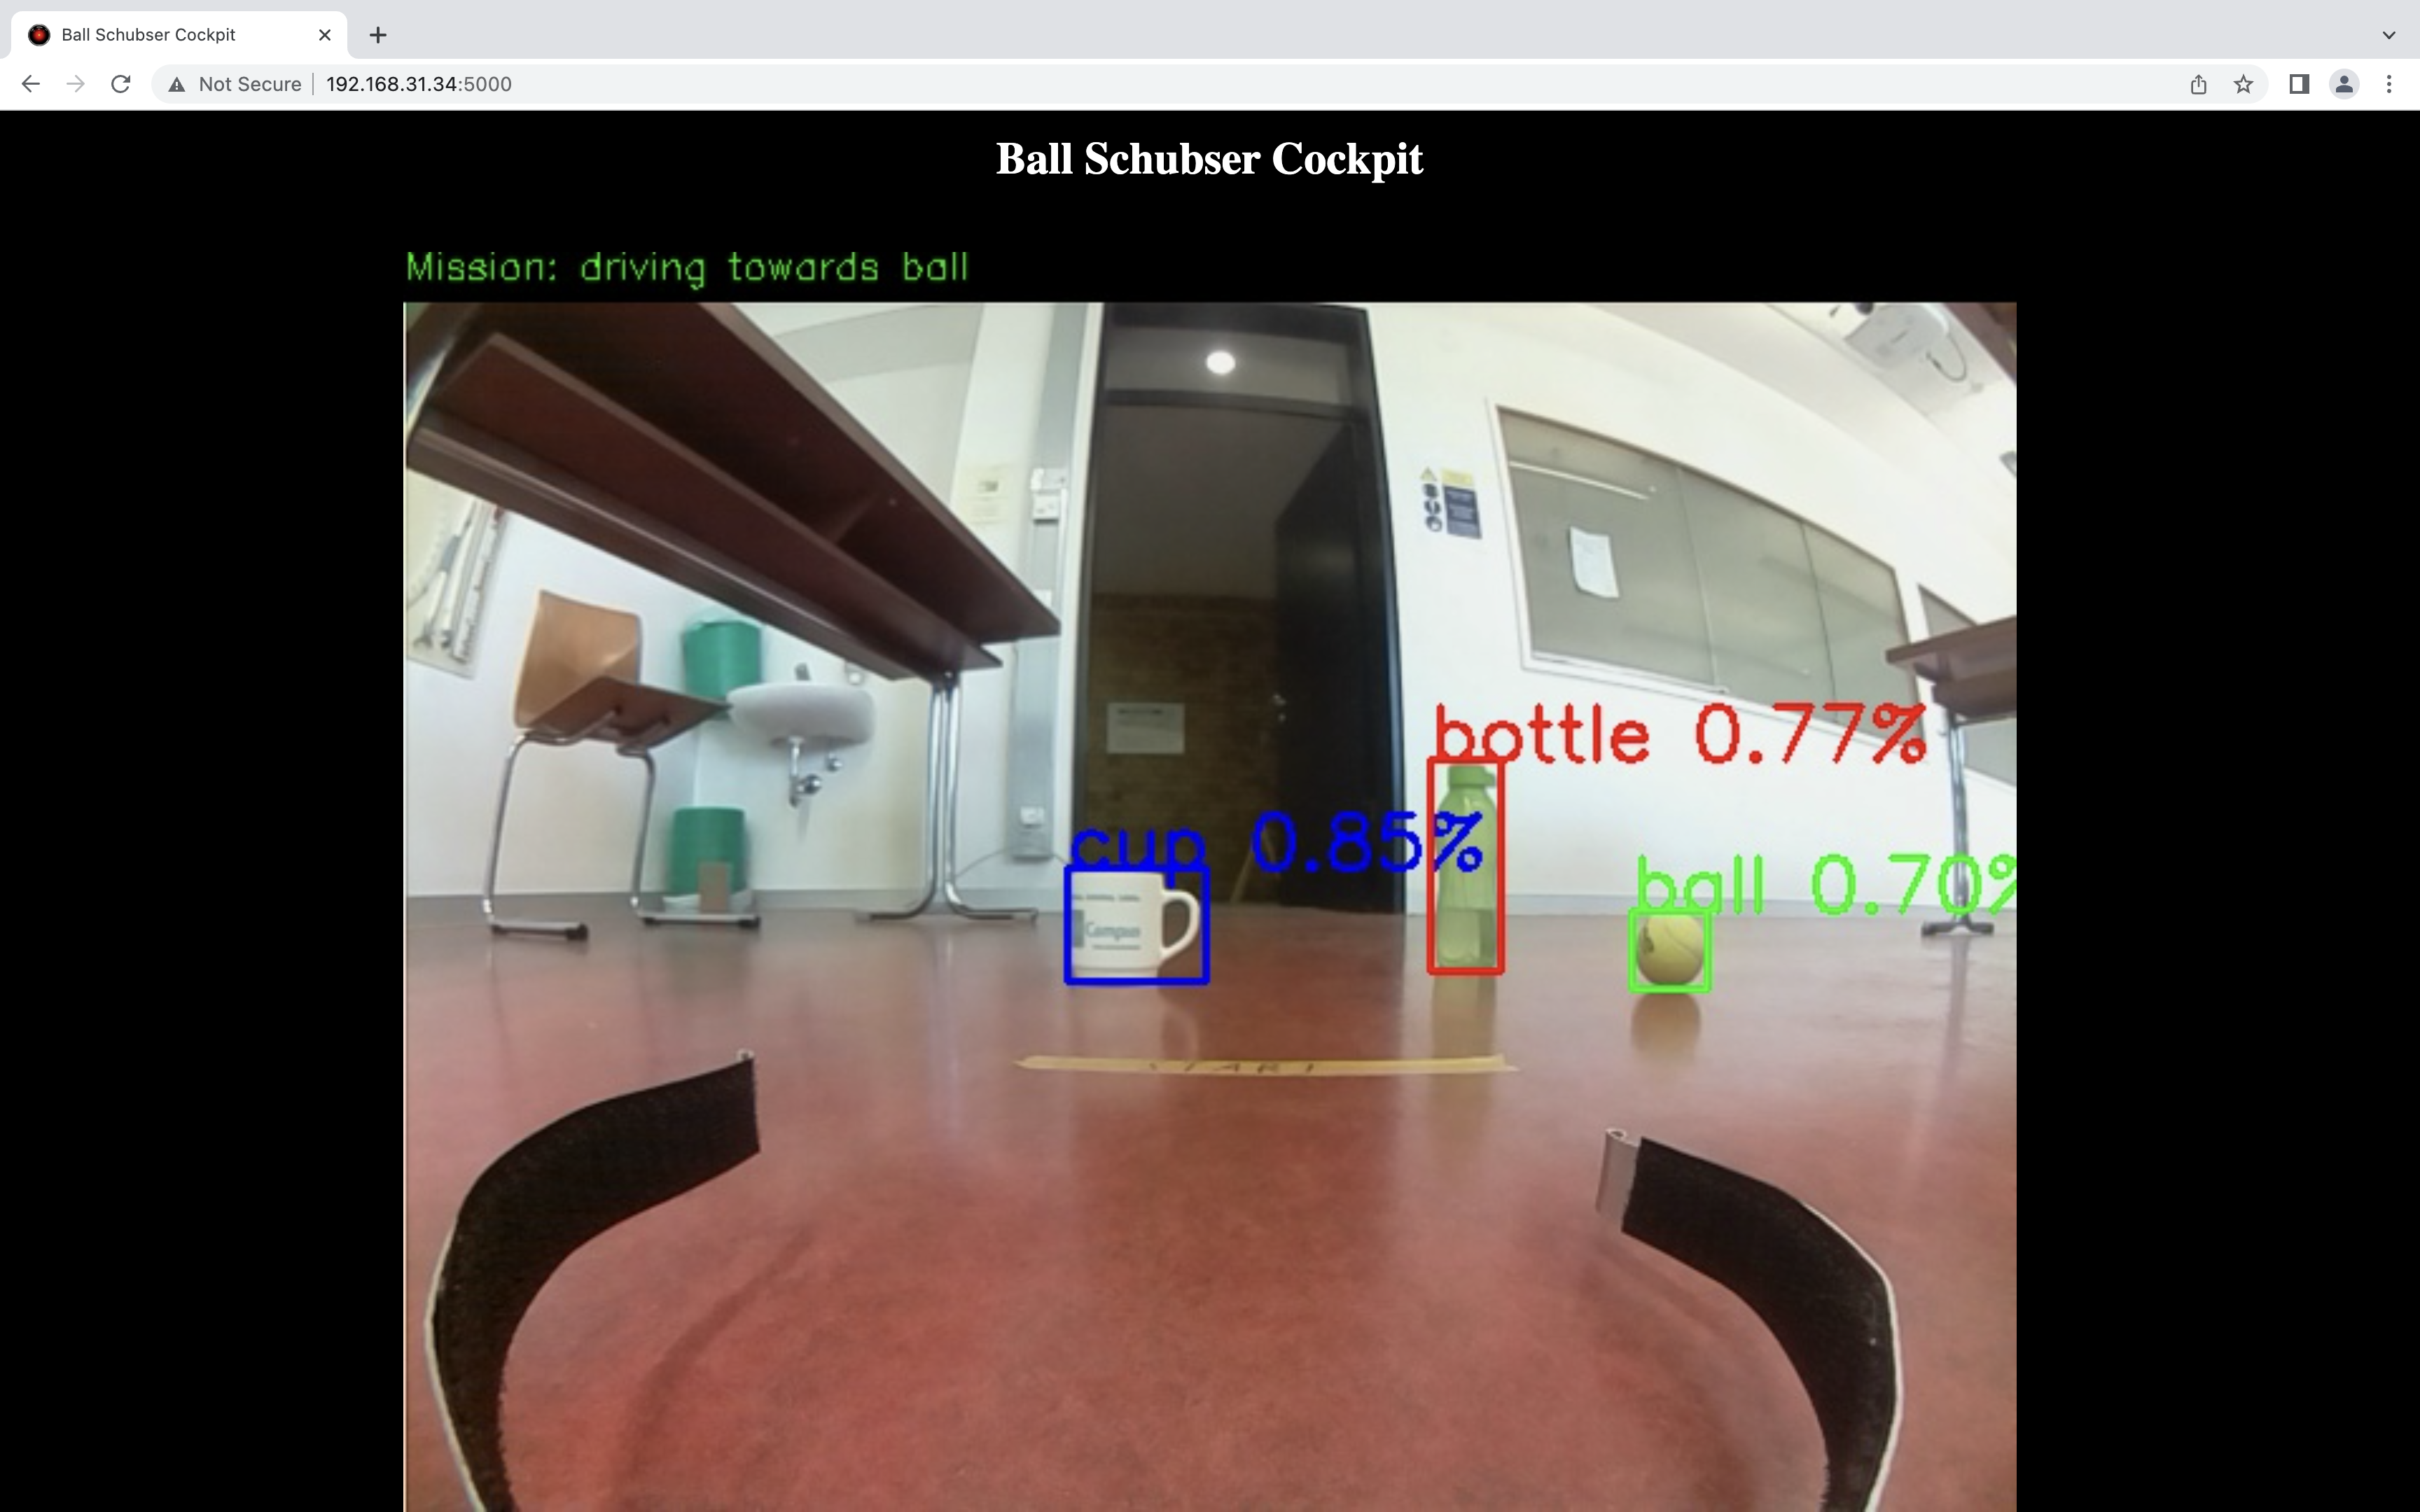
\includegraphics[width=\linewidth]{images/turtlebot-setup/cockpit.png}
\caption{Cockpit showing bounding boxes of ball, bottle and mug}
\label{fig:cockpit}
\end{figure}

The Cockpit is viewable inside the web browser and is based on Flask, a Python framework for creating web servers. Flask has different functionalities, like automatically updating the shown image when a new one is available. It enables a \enqoute{live stream} of images by always showing the latest image retrieved by the detection node through the debug\_image topic. The detection node modifies the image with bounding boxes in different colors. Each color represents a different class:

\begin{itemize}
    \item red: bottle
    \item green: ball
    \item blue: mug
\end{itemize}

The image containing the bounding boxes is then modified with a mission text published by the navigation node on the mission topic. All of the modifications on the image are done with OpenCV.

\subsection{Different Setup Approaches and Problems}

Installing large and complex software packages like \ac{ROS} and \ac{YOLO} directly onto a computer occupies a lot of space. It makes it difficult to switch between versions and to make changes to the general infrastructure setup. To solve this issue a containerized setup is implemented, besides changing the configuration, in addition this makes it easier to move the entire setup between computers.
Slow transfer rates between the remote computer and the Turtlebot do often cause malfunctions in the navigation, as the robot is receiving delayed updates from the remote computer. Moving the setup onto the Raspberry Pi didn’t bring any improvements as the computing power becomes a new bottleneck as the image processing with YOLO takes up to 6s, compared to a few milliseconds on the remote computer. So through a process of elimination, it was established that the best solution was offloading the processing job with the biggest bottleneck being the network connection. As it is not clear what exactly causes the delays on the network, no further investigations were pursued. This problem might be overcome in the future by a newer or different single-board computer e. g. the NVIDIA Jetson or a different setup with a better router, WiFi chips, and computing power. In the meantime working with a remote computer is indispensable.